\documentclass[12pt, twoside]{article}
\documentclass[12pt, twoside]{article}
\usepackage[letterpaper, margin=1in, headsep=0.2in]{geometry}
\setlength{\headheight}{0.6in}
%\usepackage[english]{babel}
\usepackage[utf8]{inputenc}
\usepackage{microtype}
\usepackage{amsmath}
\usepackage{amssymb}
%\usepackage{amsfonts}
\usepackage{siunitx} %units in math. eg 20\milli\meter
\usepackage{yhmath} % for arcs, overparenth command
\usepackage{tikz} %graphics
\usetikzlibrary{quotes, angles}
\usepackage{graphicx} %consider setting \graphicspath{{images/}}
\usepackage{parskip} %no paragraph indent
\usepackage{enumitem}
\usepackage{multicol}
\usepackage{venndiagram}

\usepackage{fancyhdr}
\pagestyle{fancy}
\fancyhf{}
\renewcommand{\headrulewidth}{0pt} % disable the underline of the header
\raggedbottom
\hfuzz=2mm %suppresses overfull box warnings

\usepackage{hyperref}
\usepackage{float}

\title{Algebra 2}
\author{Chris Huson}
\date{November 2023}

\fancyhead[LE]{\thepage}
\fancyhead[RO]{\thepage \\ Name: \hspace{4cm} \,\\}
\fancyhead[LO]{BECA / Huson / Algebra 2: Polynomials \\* 15 November 2023}

\begin{document}

\subsubsection*{2.12 Pre-Exam: Polynomial functions}
\begin{enumerate}

\subsubsection*{A1-A.APR.1 Add, subtract, and multiply polynomials}

\item Find the sum in standard form $(x^3-7x^2+2x+5)+(2x^3+9x^2-3x-5)$ \vspace{1.5cm}

\item Find the difference $f(x)-g(x)$ as a polynomial in standard form, given \\[0.25cm]
    $f(x)=x^4+2x^2-3$ and $g(x)=2x^3+2x^2-3x+3$. \vspace{2cm}

\item Multiply the two polynomials $f(x)=2x^2-3$ and $g(x)=4x^3-x+1$. First complete the grid and then collect terms to find the product as a polynomial in standard form. \\[0.25cm]
\renewcommand{\arraystretch}{2}
\begin{tabular}{|p{1cm}|p{3cm}|p{3cm}|p{3cm}|}
    \hline
     & $4x^3$ & $-x$ & $1$ \\
    \hline
    $2x$ &  & & \\
    \hline
    $-3$ &  & & \\
    \hline
\end{tabular} \vspace{3cm}

\subsubsection*{A1-A.APR.3 Identify zeros of polynomials when factorizations are available.}
\item Select all solutions to the equation $(x+1)(3x-2)=0$.
    \begin{multicols}{3}
    \begin{enumerate}
        \item $x= -\frac{3}{2}$
        \item $x= 1$
        \item $x=\frac{2}{3}$
        \item $x= -\frac{2}{3}$
        \item $x= -1$
        \item $x=\frac{3}{2}$
    \end{enumerate}
    \end{multicols}

\item Write down the solutions to the equation $x(x-3)(2x+8)(x+3)=0$. \vspace{0.5cm}

\item Write down a polynomial in factored form having roots of $x = -3, 4, 10$.

\newpage
\subsubsection*{A2-F.IF.7c Graph polynomials, identify zeros, end behavior}
\item Below is a graph of the polynomial $f(x)$. 
\begin{multicols}{2}
    What is the degree of the function?\\[1.5cm]
    Which of the following could be its equation?
    \begin{enumerate}
        \item $f(x)=(x+2)(x-4)(x-2)^2$
        \item $f(x)=(x-2)(x-4)(x+2)^2$
        \item $f(x)=(x+2)(x+4)(x-2)^2$
        \item $f(x)=(x-2)(x+4)(x+2)^2$
    \end{enumerate} \vspace{1cm} \;

    \columnbreak
    \begin{tikzpicture}[xscale=0.7, yscale=0.7]
        \draw[lightgray,very thin] (-5,-5) grid (4,5);
        \draw [thick, ->] (-5.2,0) -- (4.4,0) node [above] {$x$};
        \draw [thick, ->] (0,-5.2)--(0,5.5) node [right] {$y$};
        \foreach \x in {-5,4} \draw (\x cm,5pt) -- (\x cm,-5pt) node[below] {$\x$};
        \draw (5pt,5 cm) -- (-5pt,5 cm) node[left] {$50$};
        %\fill (-1,0) circle[radius=0.1] node[above left]{$j$};
        %\fill (3,0) circle[radius=0.1] node[above right]{$k$};
        \draw [thick, <->,smooth,samples=20,domain=-4.5:2.3] plot(\x,{0.1*(\x+4)*(\x-2)*(\x+2)^2});
    \end{tikzpicture}
\end{multicols}

\item Given the polynomial $g(x)=-2x^3-2x^2+10x-6$, graphed below. 
\begin{multicols}{2}
    \begin{enumerate}[itemsep=0.5cm]
        \item What is the leading coefficient?
        \item Write down the constant term.
        \item What are roots of the function?
        \item What factor has a multiplicity of 2?
        \item Write down the $y$-intercept as an ordered pair.
        \item What term do we use to describe the point $p$ on the plot?
        \item What is the end behavior?
    \end{enumerate} \vspace{1cm} \;

    \columnbreak
    \begin{tikzpicture}[xscale=0.7, yscale=0.7]
        \draw[lightgray,very thin] (-5,-5) grid (5,5);
        \draw [thick, ->] (-5.2,0) -- (5.2,0) node [above] {$x$};
        \draw [thick, ->] (0,-5.2)--(0,5.5) node [right] {$y$};
        \foreach \x in {-5,4} \draw (\x cm,5pt) -- (\x cm,-5pt) node[below] {$\x$};
        \draw (5pt,5 cm) -- (-5pt,5 cm) node[left] {$25$};
        \node at (0,-1.2) {$\bullet$};
        \fill (-1.67,-3.8) circle[radius=0.12] node[below left]{$p$};
        \draw [thick, <->,smooth,samples=20,domain=-3.6:2.6] plot(\x,{-0.4*(\x+3)*(\x-1)^2});
    \end{tikzpicture}
\end{multicols}

\end{enumerate}
\end{document}